% !TEX root = ./master.tex
\chapter[\'Etude clinique]{\'Etude clinique}

%Souvenons-nous brièvement de l'évolution de la signification du terme
%``clinique'' enraciné dès l'Antiquité.
%A l’origine,\textbf{ l’activité clinique} (<gr. klinê = le lit) est celle du médecin qui, au chevet du malade, procède à l’examen des manifestations de la maladie (méthode de l’observation, de l’interrogation et de l’écoute) en vue de poser un diagnostic*, un pronostic* et une prescription* de traitement.
%Michel Foucault (1926-†1984), psychologue français, dans son ouvrage capital de 1963,
%«Naissance de la clinique» nous rend attentifs au fait que l’adjectif «clinique» fut longtemps du monopole médical, avec %l’observation « naturelle » faite au lit du malade, uniquement à l’aide des organes sensoriels.

%Hippocrate (médecin grec, Cos 460-377) était clinicien : il apprenait à ses étudiants l’art d’observer les symptômes, ceux-ci étant les réactions d’une personnalité à une agression pathogène. Généralisation et rationalisation, selon les critères d’Aristote, permettaient l’élaboration de « ces entités nosologiques* », les maladies, qui s’emparaient du corps du malade et poussant les médecins, exorcistes laïques, à les en faire sortir.
%Les publications de Th.Ribot à la Sorbonne rejoignent [avec «La psychologie des sentiments »(1896), «Les maladies de la mémoire »(1883) et «Les maladies de la personnalité » (1885)], les idées de S. Freud, montrant la primauté de la vie affective, où les tendances inconscientes jouent un rôle fondamental, et pouvant s’extérioriser soit par l’arrêt du développement affectif, soit par la dissolution des acquisitions plus récentes.

%L’expression « psychologie clinique » apparaît sous la plume de S. Freud, dans sa lettre à W. Fliess du 30.01.1899 : « Maintenant, la connexion avec la psychologie, telle qu’elle se présente sur les Etudes sur l’hystérie(1895) sort du chaos, j’aperçois les relations avec le conflit, la vie, tout ce que j’aimerais appeler psychologie clinique ».

%La définition « officielle » de la psychologie clinique mobilise et articule la singularité et
%la totalité, de façon à reconnaître une discipline psychologique basée sur l’étude approfondie des cas individuels, l’étude de la conduite humaine individuelle et de ses conditions (hérédité, maturation, conditions psychologiques et pathologiques, histoire de la vie), en somme, l’étude de la personne totale «en situation», c.à.d. l’expérience vécue de ce rapport à l’environnement.

%Au vue de cet aperçu historique, on peut reconnaître que
%dans certains milieux psychiatriques actuels, la musicothérapie trouve plus sa place aussi dans le complètement des tableaux cliniques.

%Dans notre étude, l'axe principal porte sur la
%vérification de l'amélioration de
%la capacité d'écoute suite au travail musicothérapeutique.

% et procéder à la comparaison des modifications de
%l'écoute.



%\textbf{Organigramme}: nous avons obtenu l'autorisation de vous
%montrer l'organigramme de la Clinique de Meiringen lors de la
%soutenance.




%(-OH*:  le radical hydroxile, oxydrile de la molécule éthylique)



%\textbf{Le Groupe Musicothérapeutique (expérimental) GM} comporte 21
%femmes et 15 hommes.

%\textbf{Le  Groupe Contrôle GC} comporte 7 patients, dont 4 femmes et 3 hommes.

%Problème avec la comparaison et la corrélation du questionnaire avec le test d'écoute.
%Fallait-il maintenir le WQ?
%Si seulement test d'écoute
%En voulant maintenir la comparaison autant dans le nombre de WQ que de tests d'écoute
%le critère d'exclusion a été de celui d'obtenir à chaque fois le comparatif pour chaque patient
%Finalement, en tenant compte de tous ces paramètres, les participants sont au nombre de 15, tous les 
%groupes confondus:

%Afin d'obtenir une comparaison similaire tout en se basant sur la quantité de questionnaires remplis,
%de patients a dû se restreindre à
%\textbf{GM = 8 patients (4 hommes/4 femmes)
%GC = 7 patients (4 hommes/3 femmes)}


 \begin{itemize}

 \item \textbf{Nombre total de personnes}: N=  \textbf{13}:
%\textbf{Le  Groupe Contrôle GC} comporte 7 patients, dont 4 femmes et 3 hommes.

\textbf{GC: 7 : 4 femmes et 3 hommes} : Total: 14 tests pré/post
 	
\textbf{	GM: 6 : 3 hommes et 3 femmes}: Total: 12 tests pré/post
\item \textbf{Total de séances} par personne en
   musicothérapie= 4 ;   \textbf{mu}=1/semaine;
 \textbf{t}= 50--60 min, période = 3 -- 4 semaines.
  \item\textbf{Durée}: 4 semaines distribuées dans l'intervalle juin -- octobre 2017.
 \item\textbf{Genre et âge de la population étudiée:}  de 25 à 72
 ans dont l'âge moyen est de 48 ans.
 %19 hommes et 10 femmes,
 \item\textbf{Total  des test d'écoute: 26}
 \item\textbf{Total des questionnaires: 9}
\end{itemize}


\begin{figure}
	\centering
	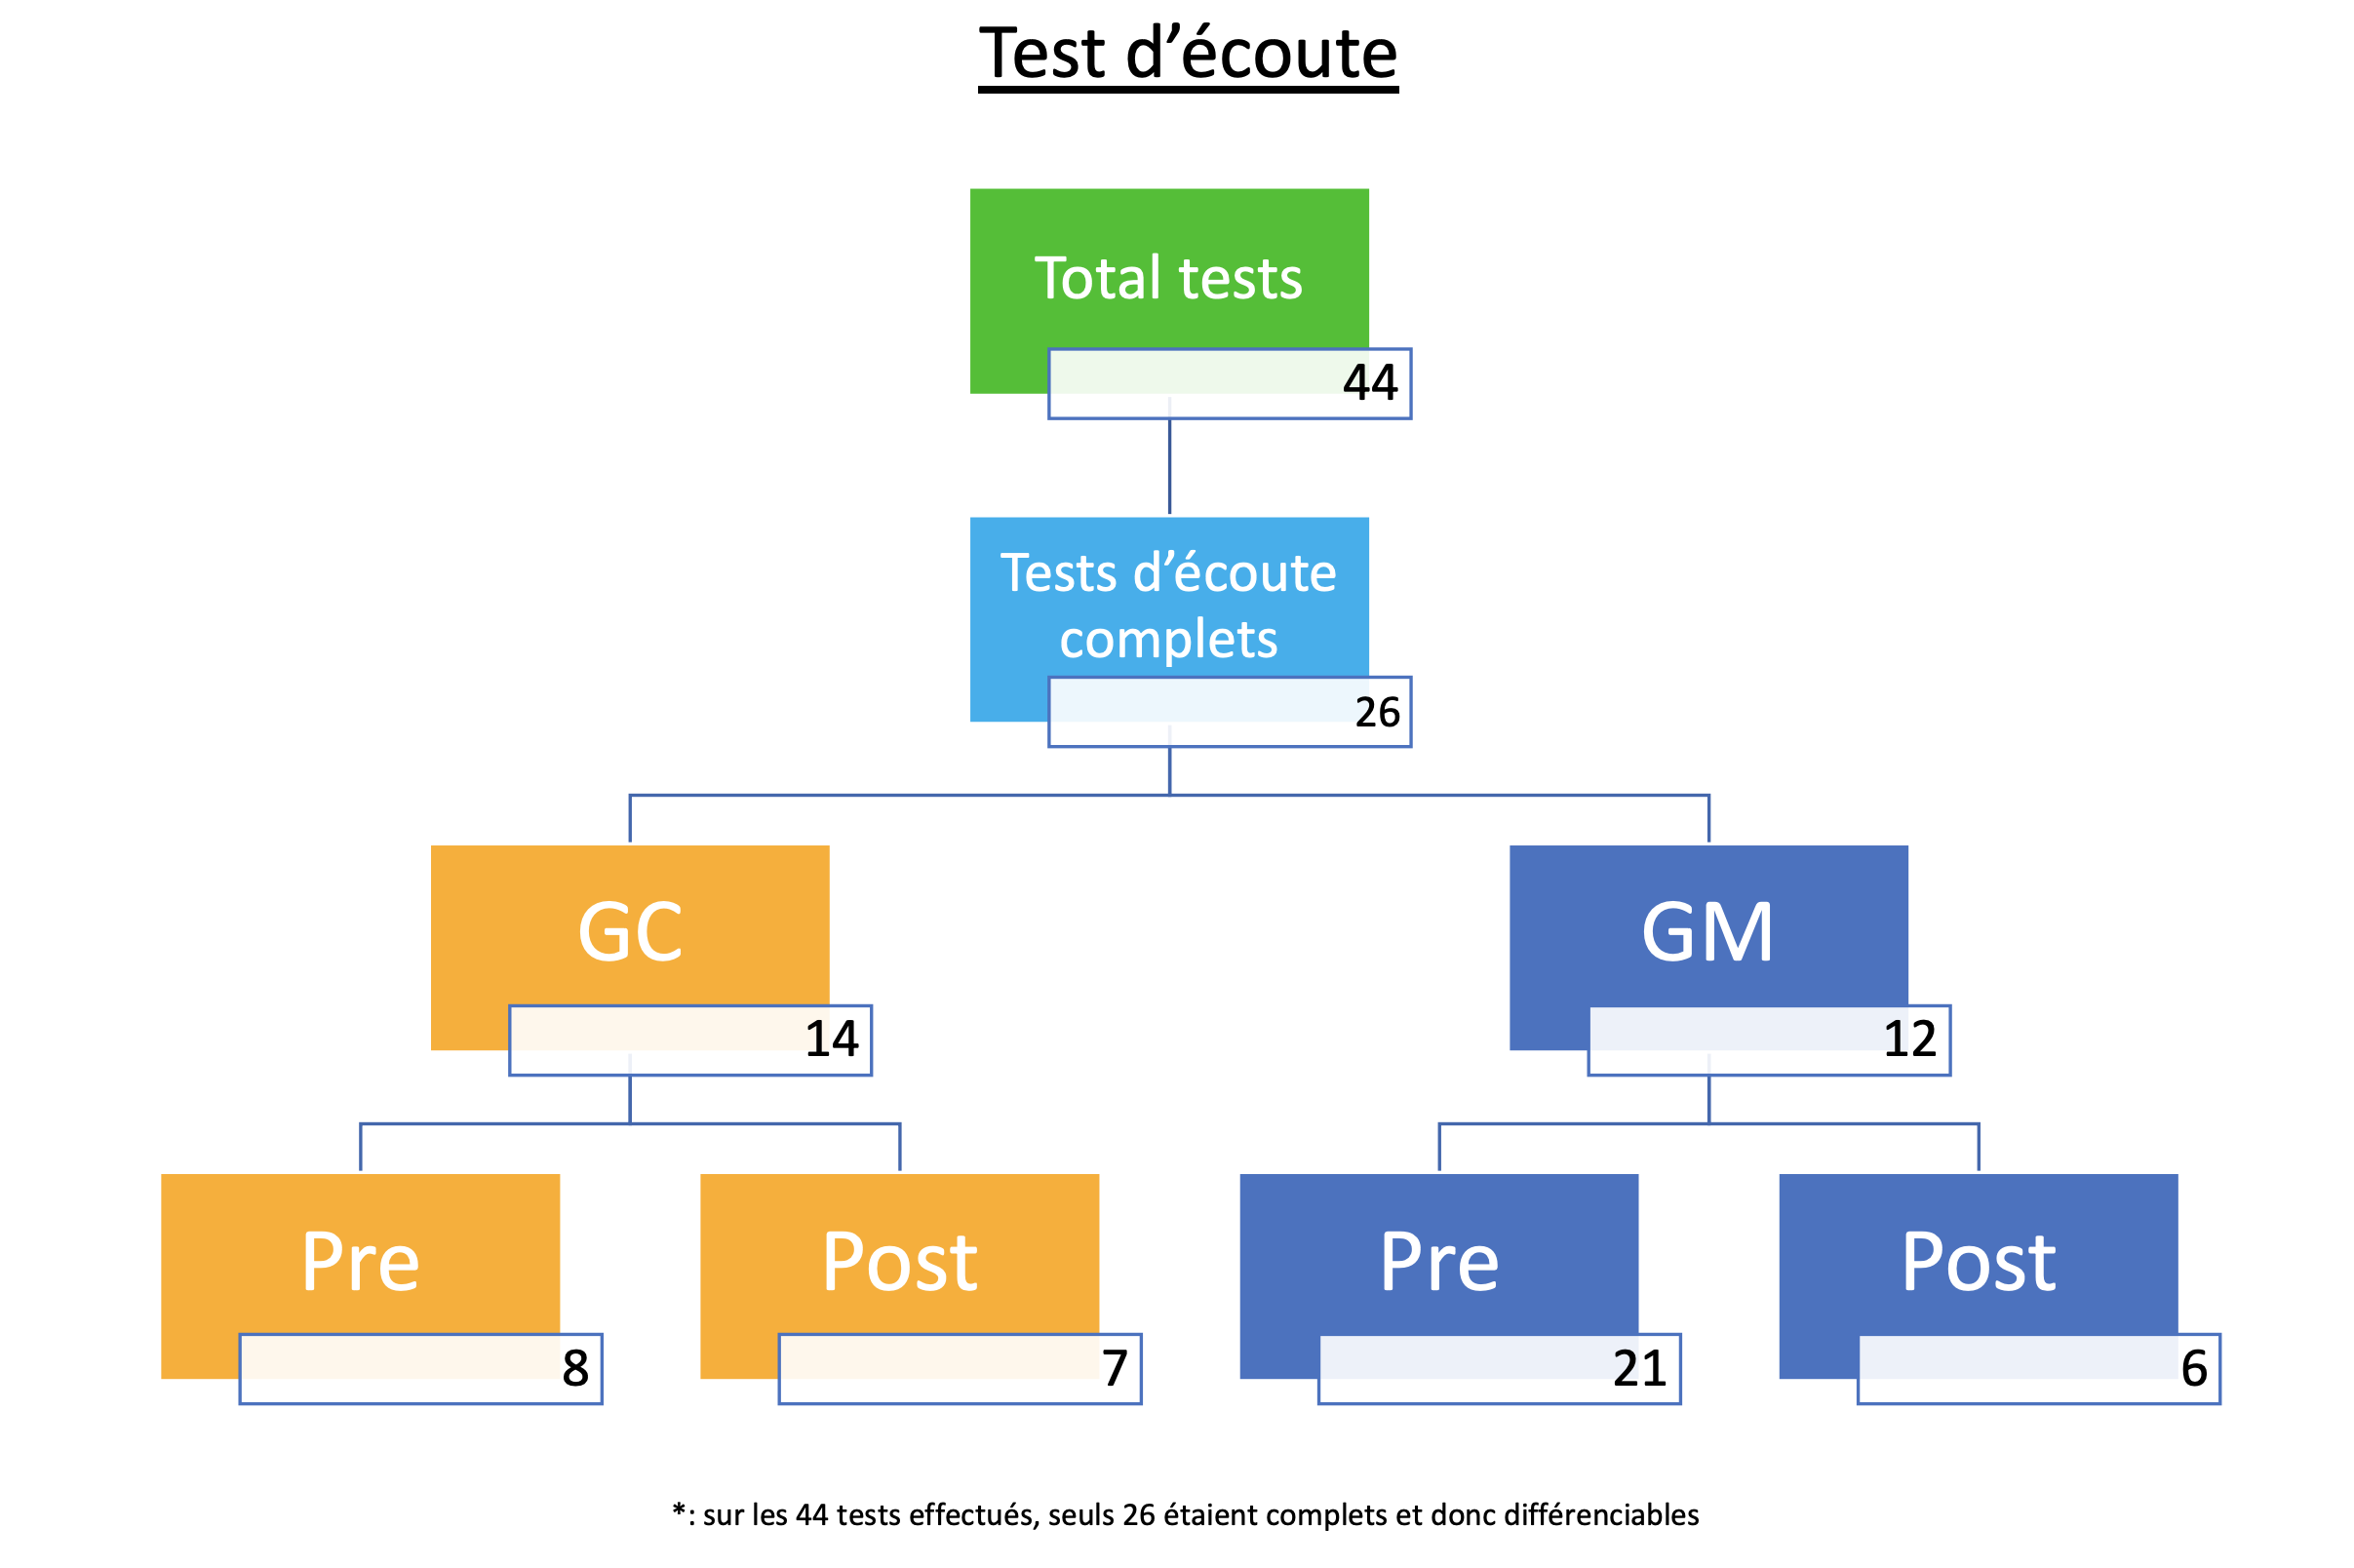
\includegraphics[width=1\linewidth]{images/graphiques/Testecoute.png}
	\caption{Nombre de tests d'écoute avec GM et GC}
	
	%\label{groupecontroleimage1}
\end{figure}



\begin{figure}
	\centering
	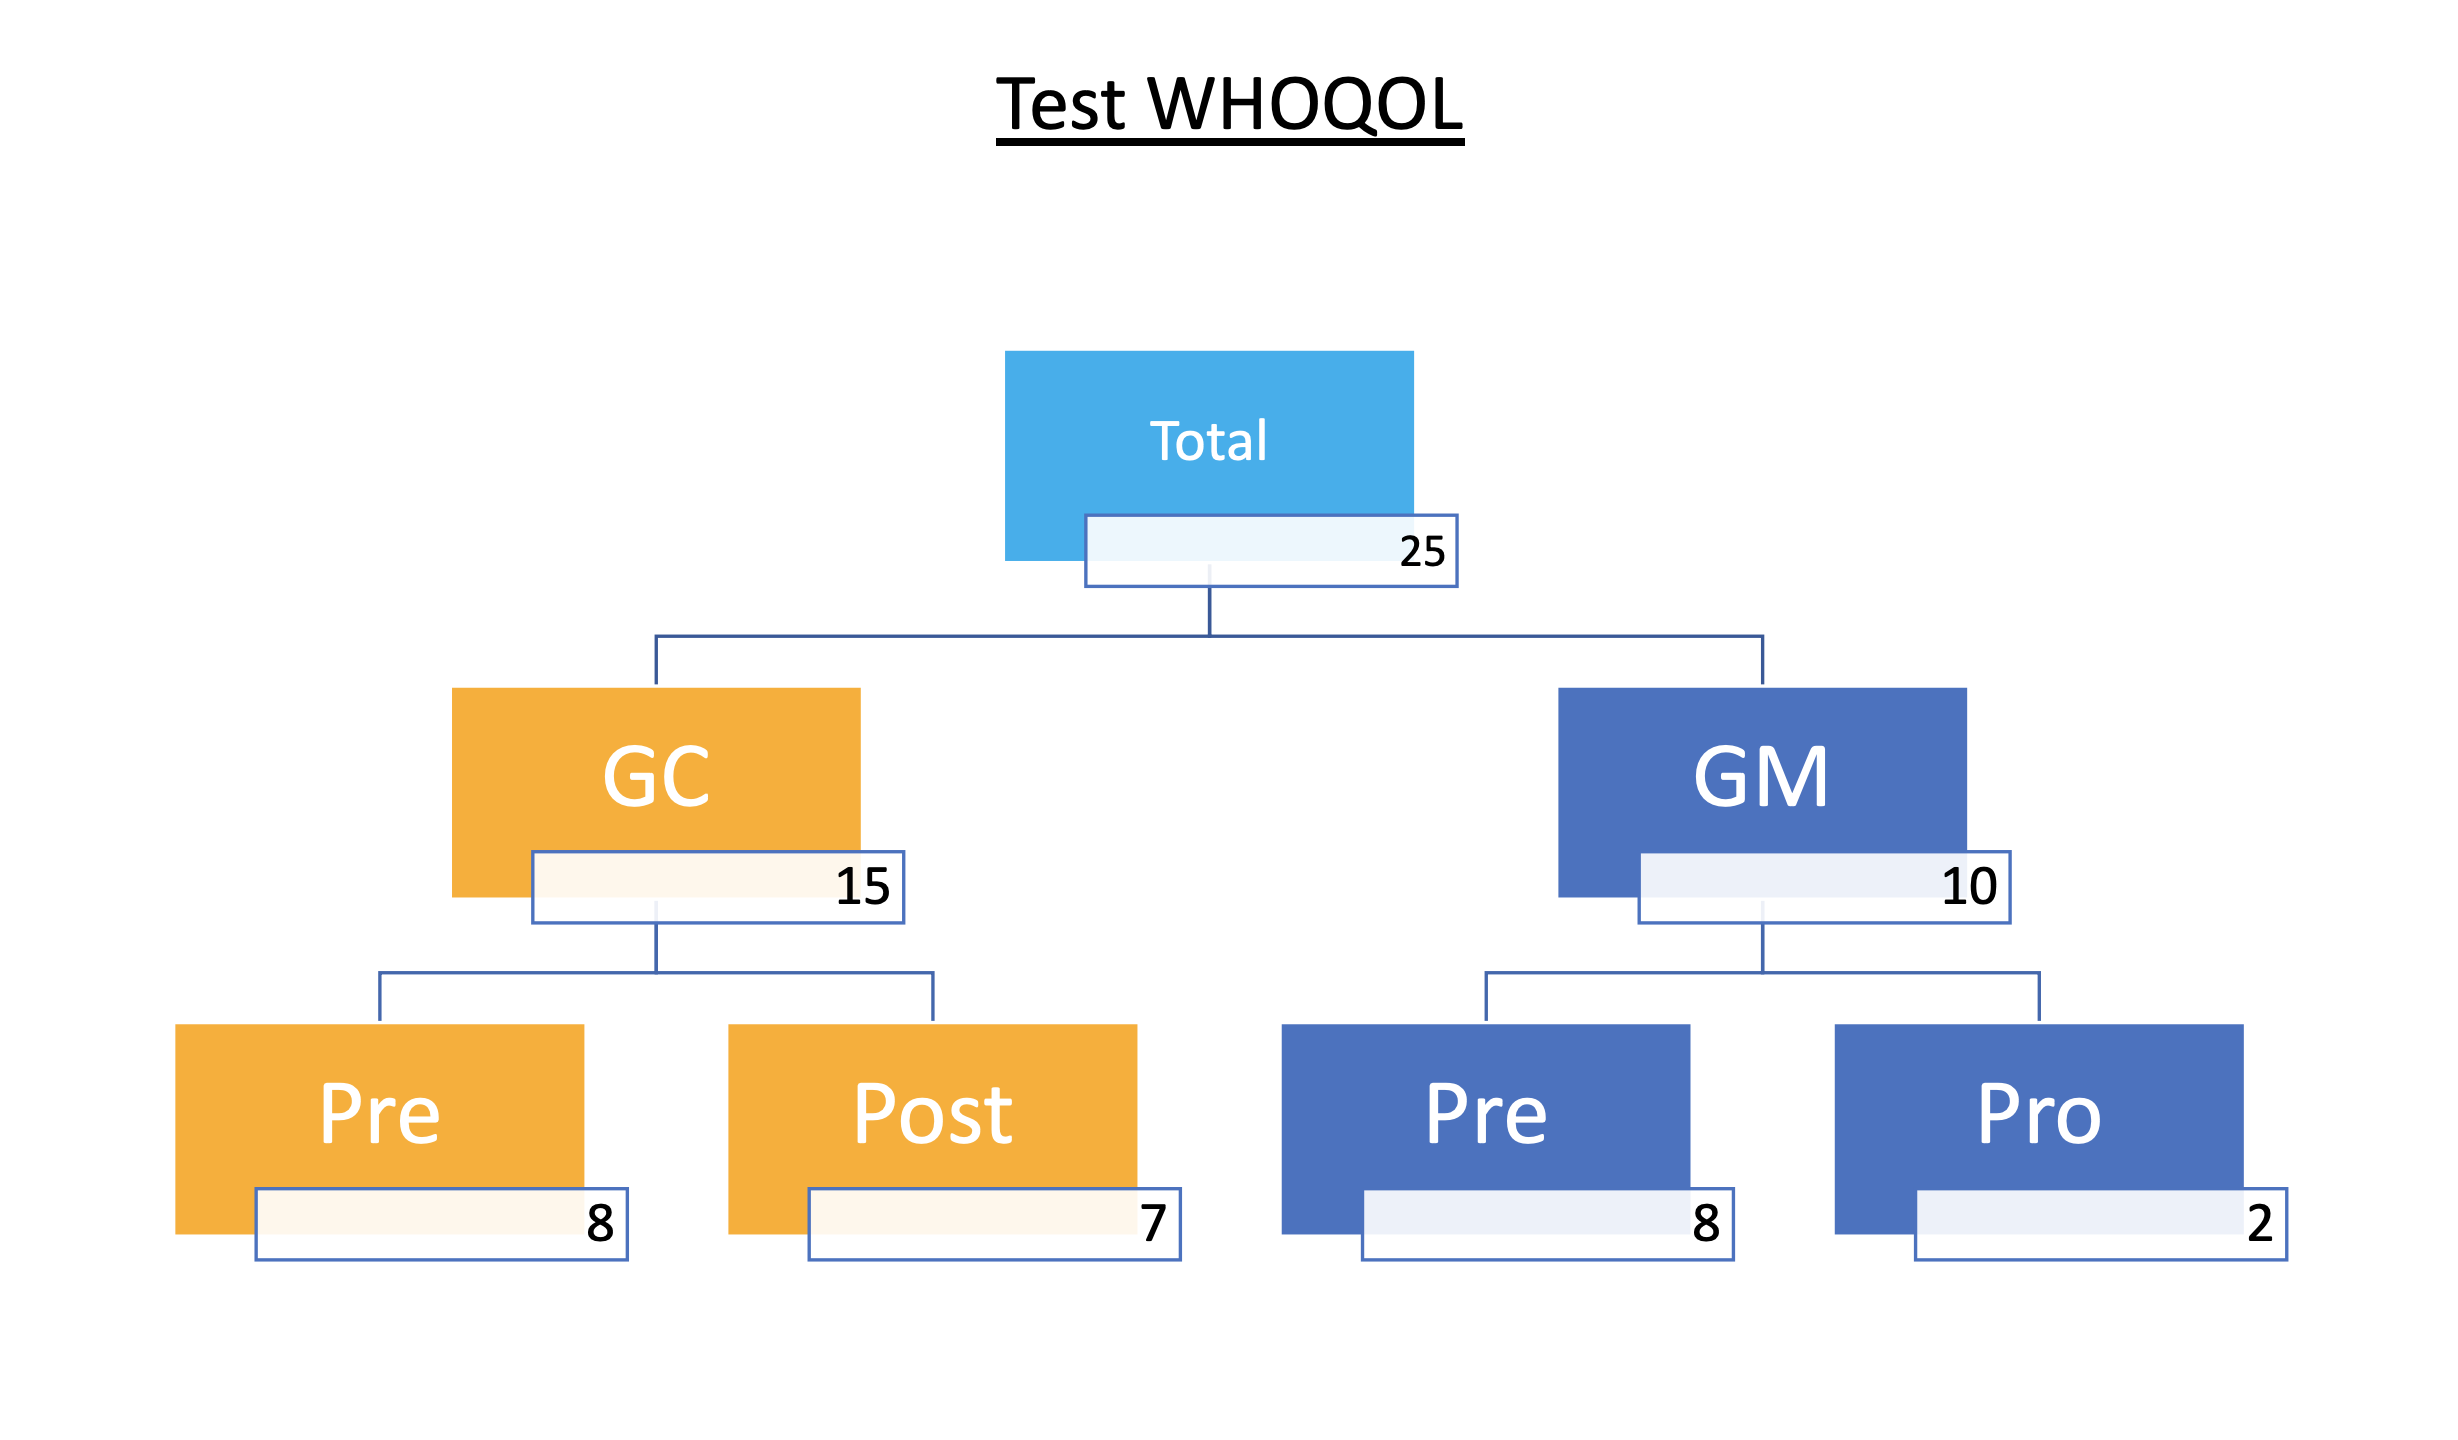
\includegraphics[width=1\linewidth]{images/graphiques/TestWQ.png}
	\caption{Nombre de WHOQOL avec GM et GC}
\end{figure}



 %mu en grec


%Après ces prémisses, l'étude commence véritablement avec l'application du test
%audiométrique suivie du questionnaire qualitatif.

    
     
     % Cela nous a 
     %conduit à 
     %la difficulté d'obtenir un nombre égal pour comparer.
     Le nombre de tests d'écoute a été presque obtenu dans sa totalité pour les 2 groupes mais 
     pas 
     pour le questionnaire: un nombre insuffisant  de WQ en fin de 
     séjour dans le groupe de musicothérapie.
     Cette  incidence a réduit considérablement la démonstration de cas proposés.
     %Nous nous sommes donc tenus à notre plan, constatant ces données  manquantes.
     En maintenant nos objectifs, c. à. dire  le comparatif autant  dans le nombre de WQ que dans le  tests 
      d'écoute, 
     %le critère d'exclusion a été de celui d'obtenir à chaque fois le comparatif pour chaque patient
     %Finalement, en tenant compte de tous ces paramètres,
     nous obtiendrons pour  les deux groupes confondus, \textbf{13 patients, 7 pour le groupe de contrôle 
     et 
     	6 pour 
     	le groupe de musicothérapie.}
     Sur \textbf{25 questionnaires WHOQOL}, il y en aura  \textbf{15 pour GC} dont 8 pré-
     et 7 post-thérapie et  \textbf{10 pour GM} remplis
     avec 8  pré- mais seulement 2
     post- thérapies:  nous aurons donc dans l'ensemble un total de \textbf{9 questionnaires} pour le
     comparatif des 2 groupes réunis.
    % Si statistique il y aurait, la survie ne serait pas élevée.
   
   
   
   Il convient ainsi de mentionner, vu la taille réduite des échantillons, qu'il n'est pas
   pertinent de se lancer dans une analyse purement
   quantitative.
   Les données que nous obtiendrons seront des valeurs indicatives.
   %dû entre autres à un très petit nombre 
   %de
   % questionnaires WQ remplis en fin de séjour pour le groupe de musicothérapie. 
   Toutefois, nous avons tenu à décrire exactement le déroulement de cette étude. Nous avons 
   décortiqué 
   tous les questionnaires et étudié tous les tests d'écoute des deux groupes.
   Avec le questionnaire 
   WHOQOL,  il  s'agira d'un analyse qualitative avec des résultats chiffrés, mais ici dans ce contexte
   statistiquement pas évaluable. 
   Avec le test d'écoute, nous obtiendrons des valeurs quantitatives sur la qualité de l'écoute, illustrés 
   par 
   des tableaux.
   Dans son ensemble, l'analyse sera considérée comme quantitative  et qualitative.
   
   
   
   \section{Questionnaires WHOQOL}
  % \section*
   \textbf{Le comparatif pré/post-thérapie:}
   nous avons mis en détail, afin que notre procédure soit claire, un comparatif entre des patients du 
   groupe de contrôle et du groupe de 
   musicothérapie dont  seuls deux du GM étaient valides car remplis en fin de thérapie. Nous aurons la 
   totalité des 
   résultats Fig. 5.1, 5.2, 5.3.
   %le patient Cav est  mentionné pour exemple de preuve de l'inexistence du questionnaire rempli en fin 
   %de 
   %thérapie) .
   %A la fin, nous avons illustré en couleur (Fig. 5.16) les
   %résultats finaux des deux groupes au complet avec 2 schémas
  % comparatifs.
   %\section*
   \paragraph{Groupe Contrôle: observation des résultats}
   %\paragraph{ GC: Représentation des résultats avec 3 patients du groupe contrôle:}
   : voici les exemples de trois patients qui ont rempli toutes les conditions de l'étude.
   \begin{enumerate}
   	\item : A. Patient Br.:  25/27 - 21/22 - 12/11 - 33/32 : $-$
   	
   	Résultat: 21,6 contre 23 pré-traitement,  ce qui
   	correspond au signe négatif.
   	\item : B. Patient Sch.: 30/27 - 20/20 -  10/10 - 35/30 :  $-$
   	
   	Résultat: 21,75 contre 23,75 pré-traitement, ce qui
   	correspond au signe négatif.
   	
   	\item :  C. Patient Wal. : 24/19 -  17/18 - 6/5 -
   	27/20 :   $-$
   	
   	Résultat: 15,5 contre 18,5 pré-traitement, ce qui
   	correspond au signe \textbf{négatif:  $-$}.
   \end{enumerate}
   
   
   \textbf{ Résultats }: les résultats présentés sont  \textbf{négatifs} 
   et confirment le ressenti subjectif moyen de l'ensemble des patients
   GC post-traitement,  comme nous le verrons avec  le résultat final  (Fig. 5.13) de
   cinq patients:  \textbf{négatif:  $-$} et deux patients:  \textbf{positif:  $+$}.
   
% \section*
\paragraph {Groupe Musicothérapie: observation des résultats}
: il ne s'agira ici que de  deux patients car ce sont les seuls qui ont rempli toutes les conditions de 
l'étude, 
 c'est-à-dire y compris celle de remplir le questionnaire en fin de séjour.
 %\paragraph{ GM: Représentation de résultats avec 2 patients du groupe de musicothérapie}
 
 \begin{enumerate}
 	\item : A. Patient Sw. : 26/25 - 19/19 - 8/8 - 29/30 :   $=$
 	
 	
 	
 	Résultat: 20,5 contre 20,5 pré-traitement, ce qui
 	correspond au signe égal.
 	
 	
 	
 	\item : B. Patient M. : 17/27 - 13/23 -  9/10 - 24/32 :  $++$
 	
 	Résultat: 23 contre 15,75 pré-traitement, correspondant
 	au signe \textbf{positif: $+$}
 \end{enumerate}
 \textbf{ Résultat final}: les résultats sont \textbf{positifs}.
 Ainsi,  GM s'exprime
 \textbf{positivement}
 sur l'ensemble du séjour en clinique, résultat très relatif, vu le petit nombre, ne pouvant être  
 représentatif du 
 groupe de 
 musicothérapie.
 Voici en résumé (Fig. 5.3) le schéma représentant la moyenne pré/post traitement, calculée pour chaque 
 patient, des scores des 4 domaines.
 
 
 \begin{sidewaysfigure}
 	\centering
 	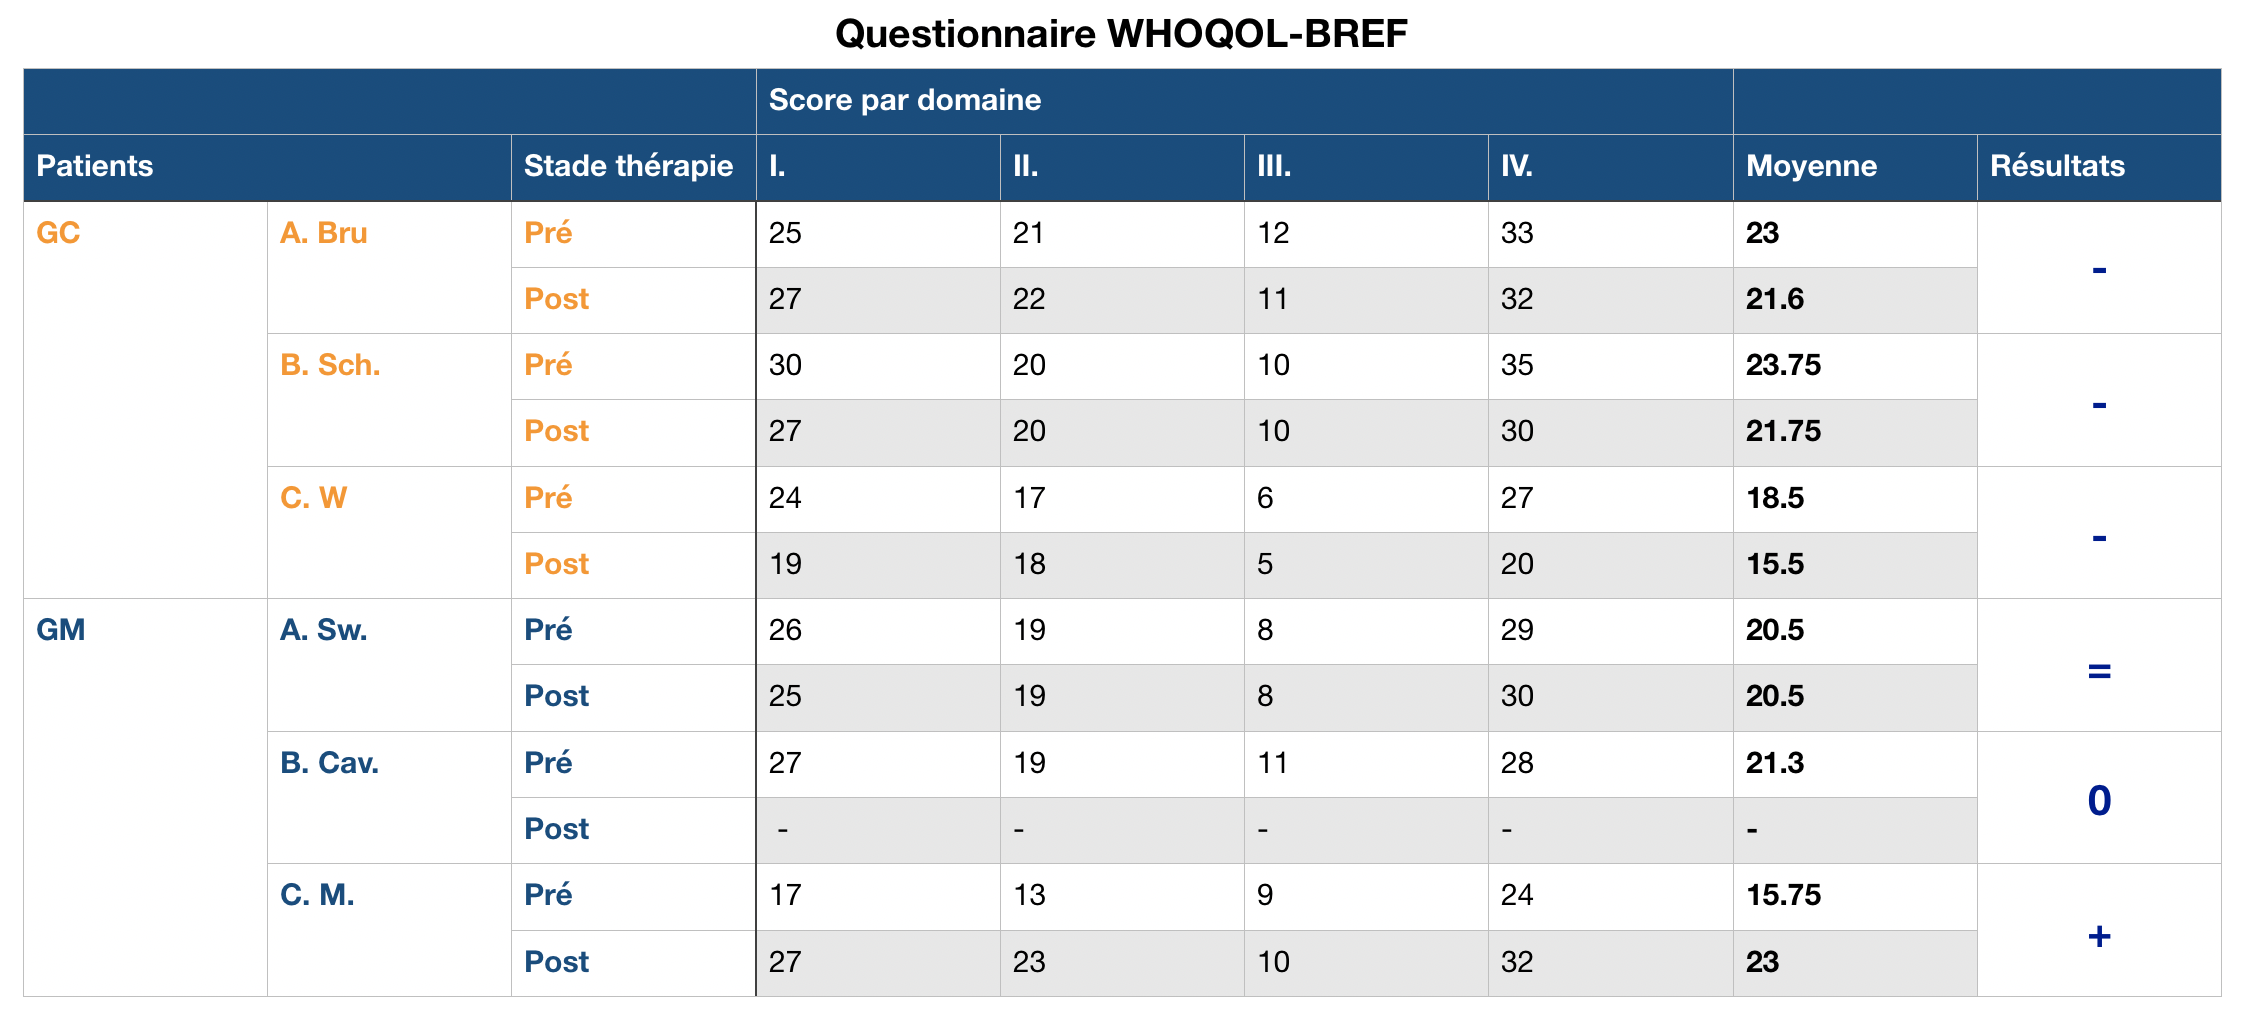
\includegraphics[width=\linewidth]{images/graphiques/questionnaire_wq.png}
 	\caption[Questionnaire WHOQOL-BREF]{GM/GC - Pré/Post avec la moyenne des scores par 
 		domaine}
 	
 	%\label{groupecontroleimage1}
 \end{sidewaysfigure}
 
 %Les chiffres ont été obtenus à partir des 4
 %domaines, avec le pré/post-séjour.
 
 
 
 
 %\section*
 \paragraph{Questionnaires WHOQOL: total des résultats du 
 	comparatif pré- / post- thé\-ra\-pie}
 
 
 
 \begin{figure} [th]
 	\centering
 	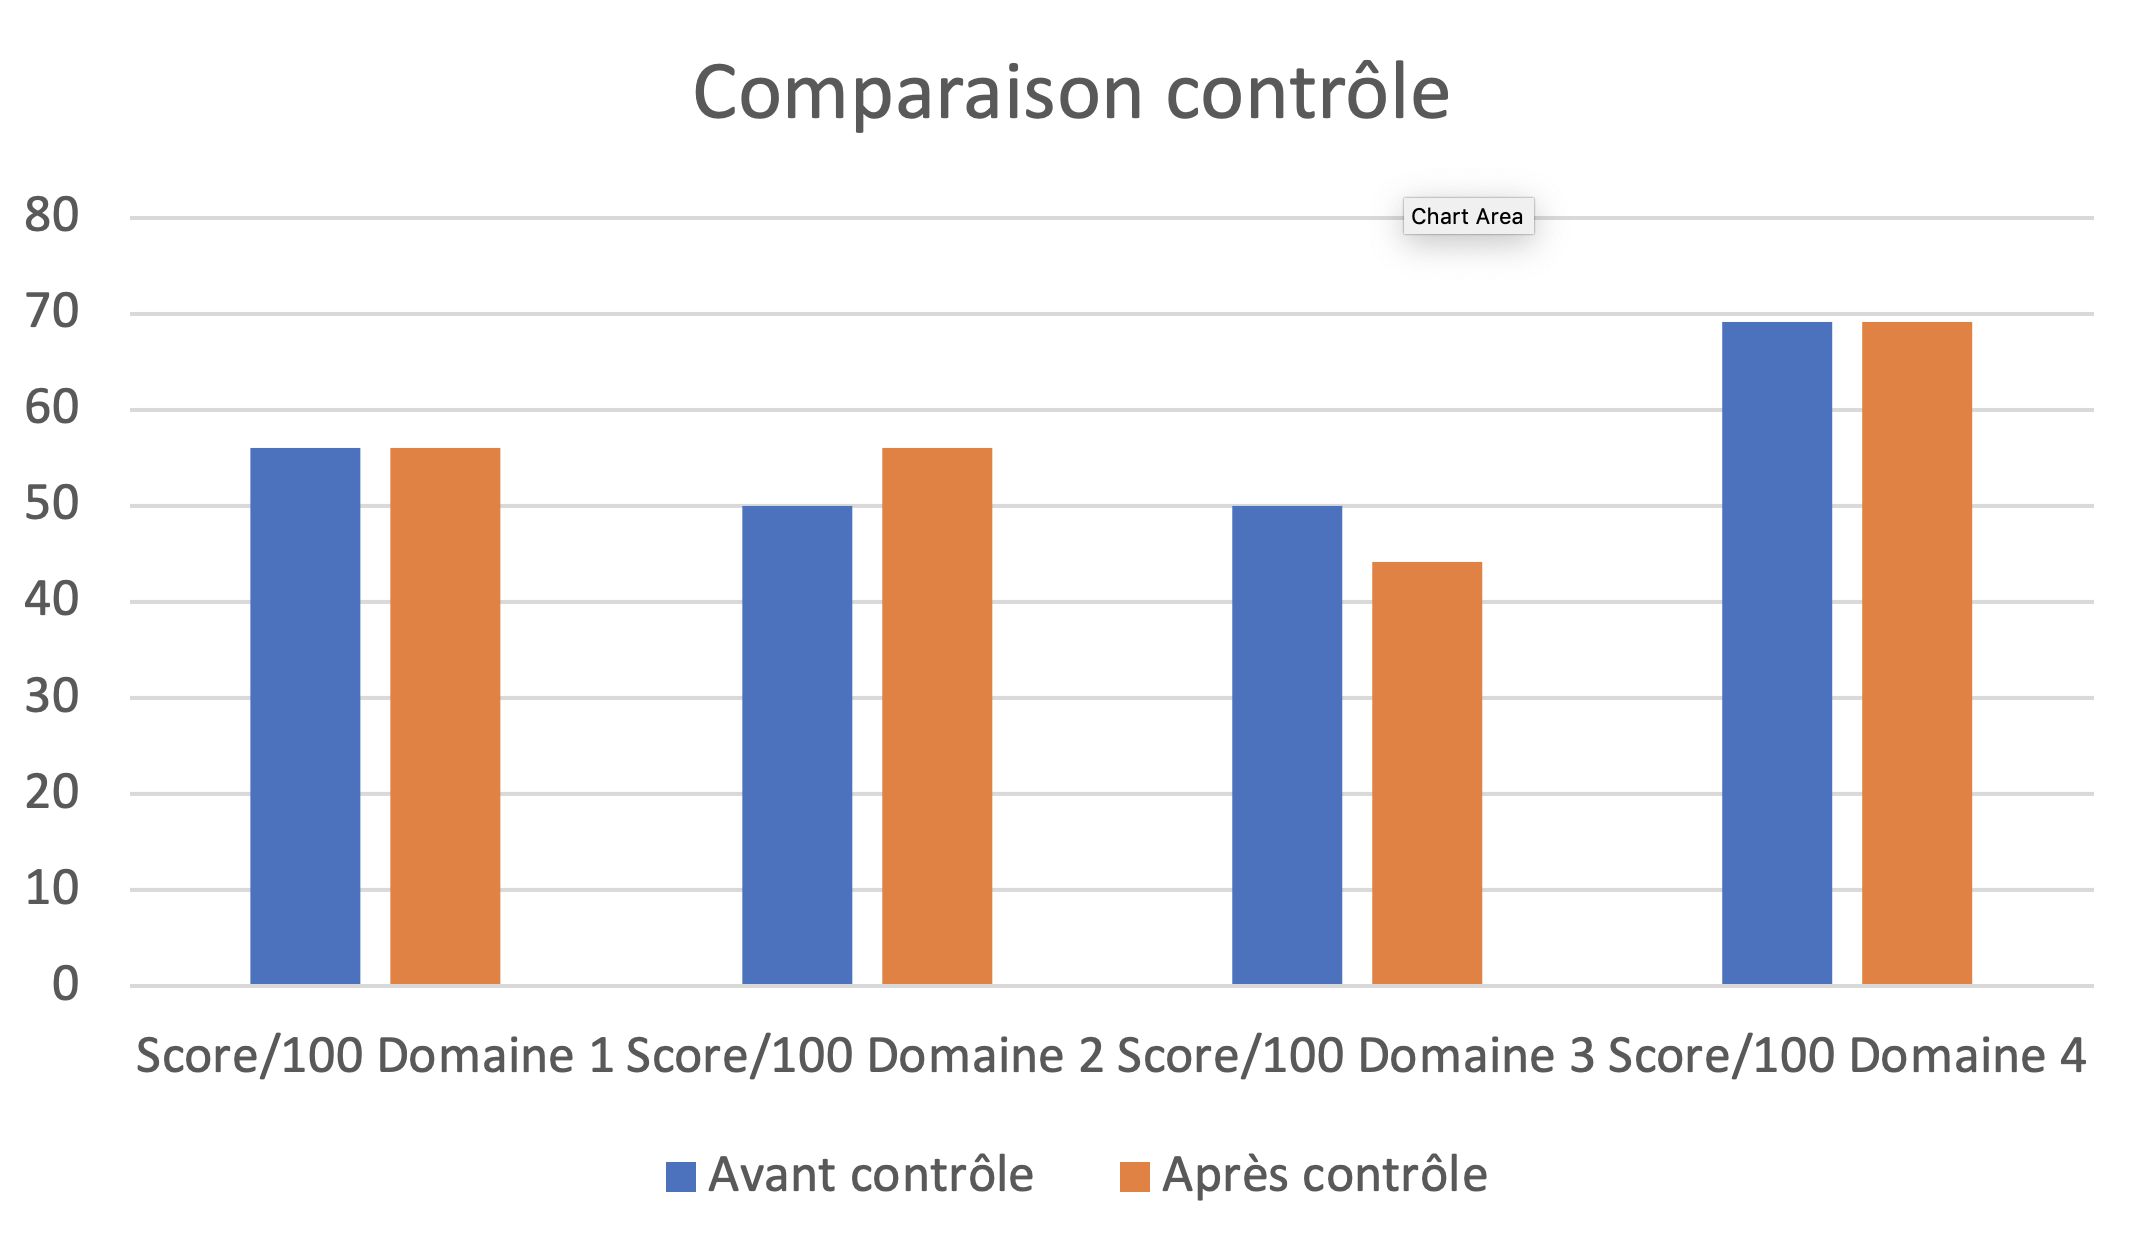
\includegraphics[width=\linewidth]{images/Compcontrole.png}
 	\caption[Schéma du déroulement]{WHOQOL:  GC. Comparatif pré/post-traitement, avec 7 patients}
 	
 	%\label{groupecontroleimage1}
 \end{figure}
 
 \begin{figure}[th]
 	\centering
 	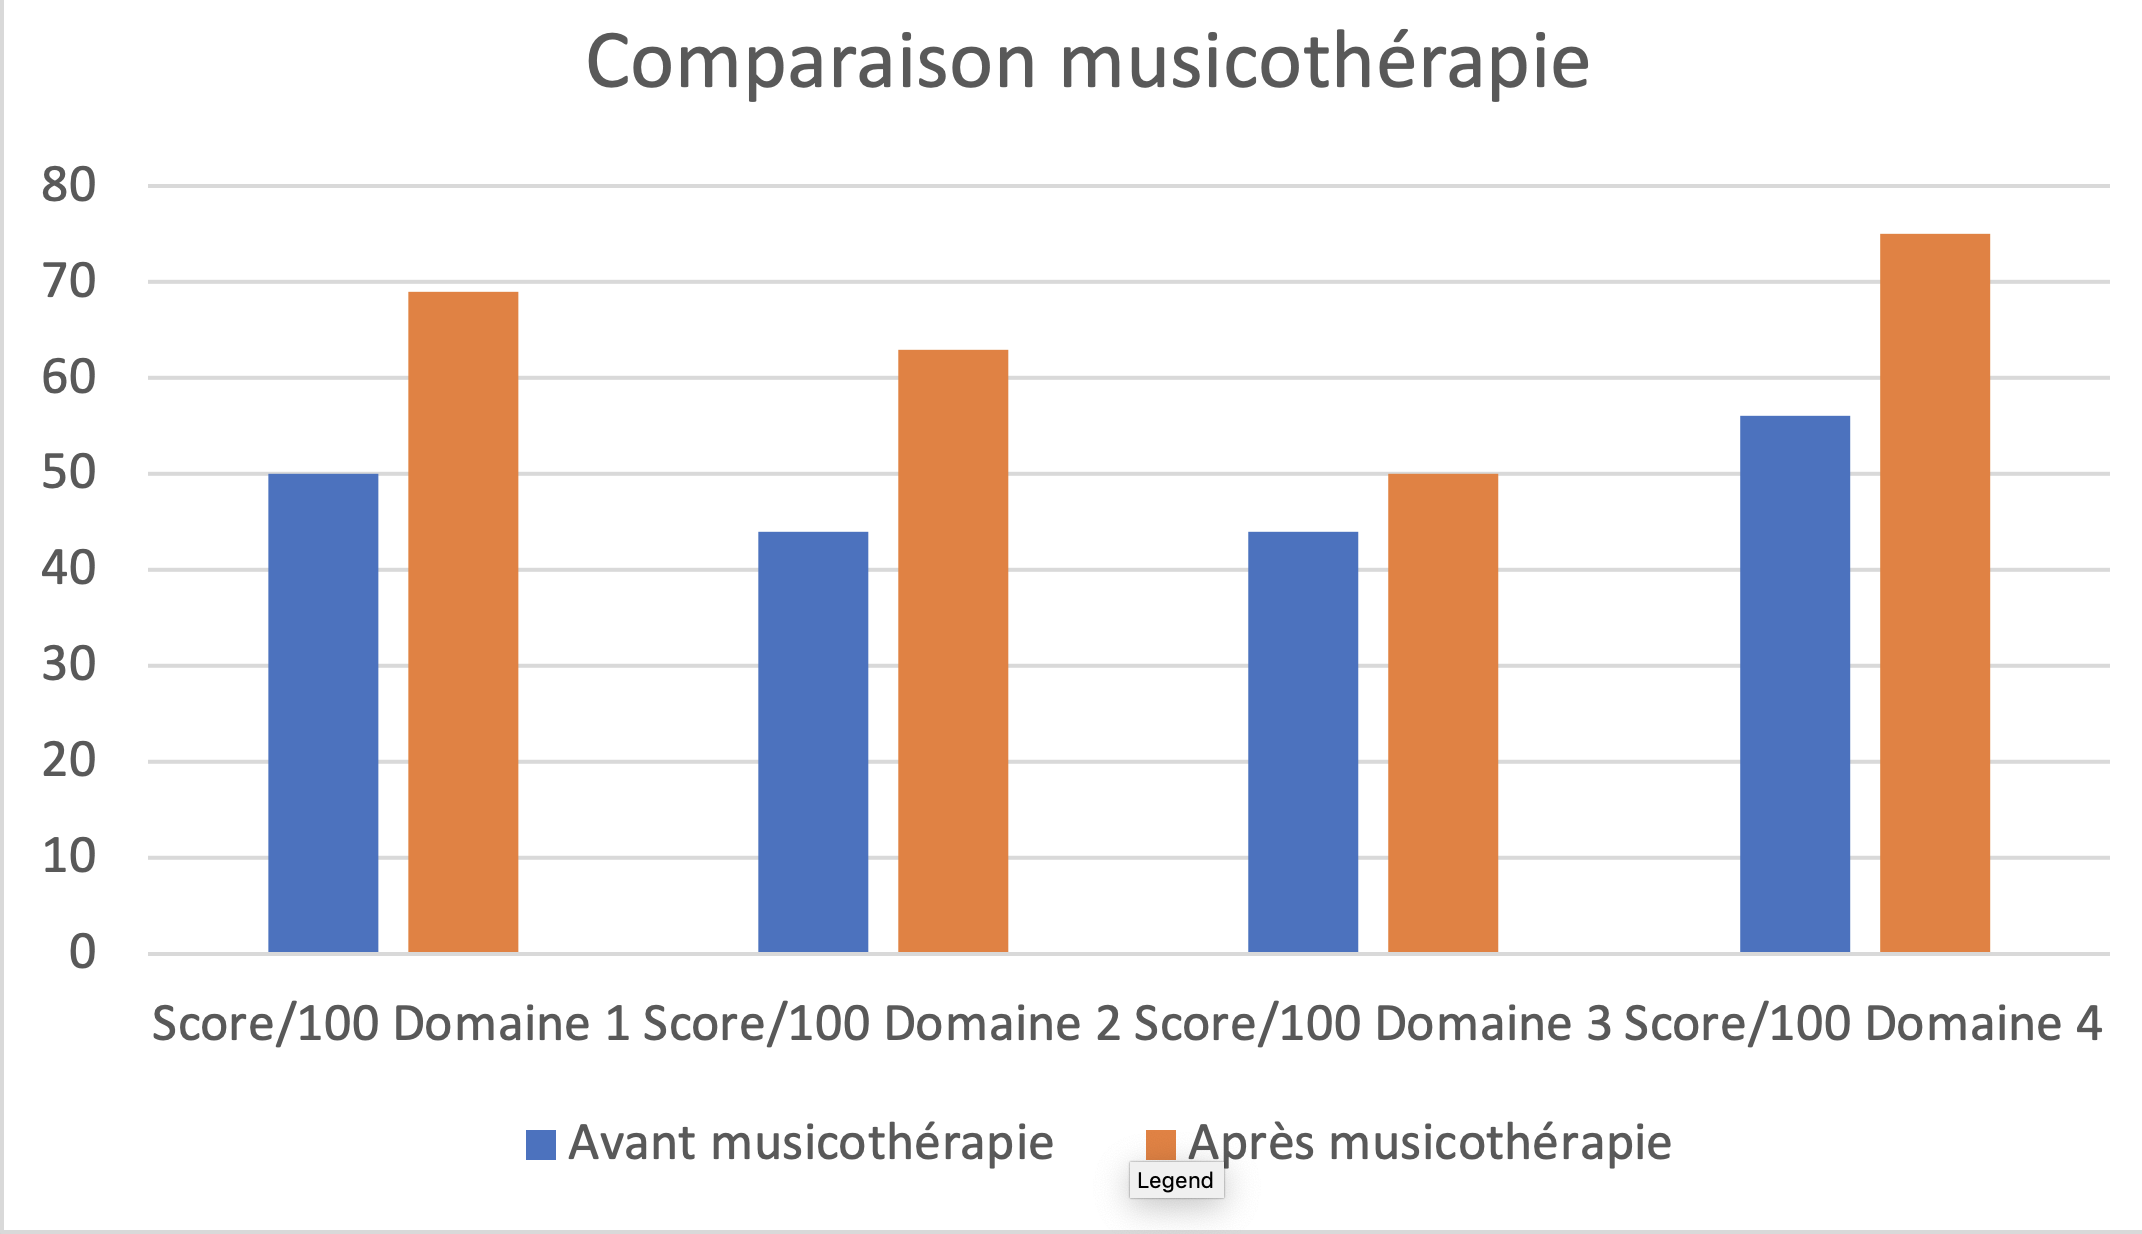
\includegraphics[width=1.0\linewidth]{images/Compmusico.png}
 	\caption[Schéma du déroulement]{ WHOQOL: GM. Comparatif pré/post-traitement avec 2 patients}
 	
 	%\label{groupecontroleimage1}
 \end{figure}
 
 
 Nous avons créé un schéma des résultats des questionnaires
 pré/post-traitement du groupe de contrôle, puis du groupe de musicothérapie,
 qui  se trouve sous les Fig. 5.3/ 5.4/ 5.5.
 En résumé, nous observons selon les chiffres obtenus que  le ressenti
 subjectif d'amélioration psychique
 des patients suivis en musicothérapie apparait comme
 supérieur.
 De manière générale, l'ensemble des données des deux groupes représentés
 corrobore ce résultat.
 Ces données sont des valeurs indicatives car nous avons conscience que le petit échantillonnage ne
 peut être représentatif.

 
 \clearpage

 \section{Test d'écoute}
 % \subsection*
  \paragraph{Comparatif pré/post-thérapie:}
  %Avant d'aborder la synthèse des résultats avec la
 % \textbf{corrélation test d'écoute et questionnaire}, nous avons réuni et rassemblé sous un seul 
 %chapitre tous les autres tests d'écoute.
 pour une comparaison simplifiée et mise en parallèle avec le WQ, nous avons pris les mêmes   
 patients du GC et du GM. Avec GM, nous avons rajouté  le patient Cav et spécifié l'absence de 
 questionnaire final.
 Tous les autres seront visibles et résumés à la figure 6.1.
 \subsection*{Groupe Contrôle: observation}
  % \textbf{Groupe Contrôle: }
  \paragraph{ Patient Br.:}
  \begin{figure}[ht]
\centering
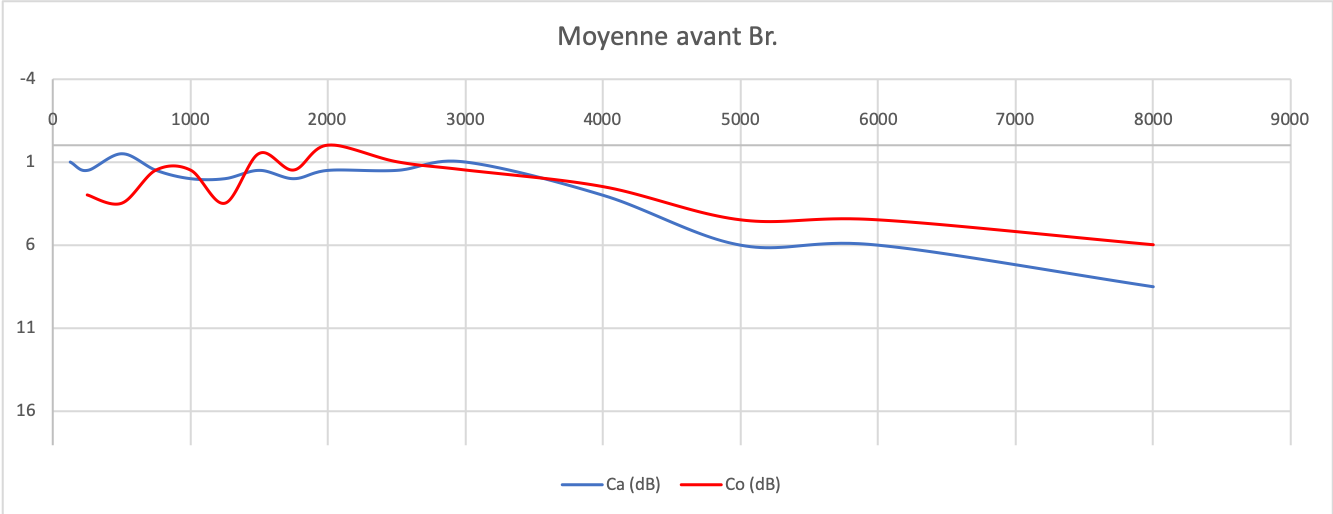
\includegraphics[width=1\linewidth]{images/graphiques/bru_pre.png}
\caption[  \textbf{Groupe Contrôle}: Patient Br.. 1° test]{Premier test Br.}
%moyenne OG et OD
%\label{groupecontroleimage1}
\end{figure}



 \begin{figure}[th]
\centering
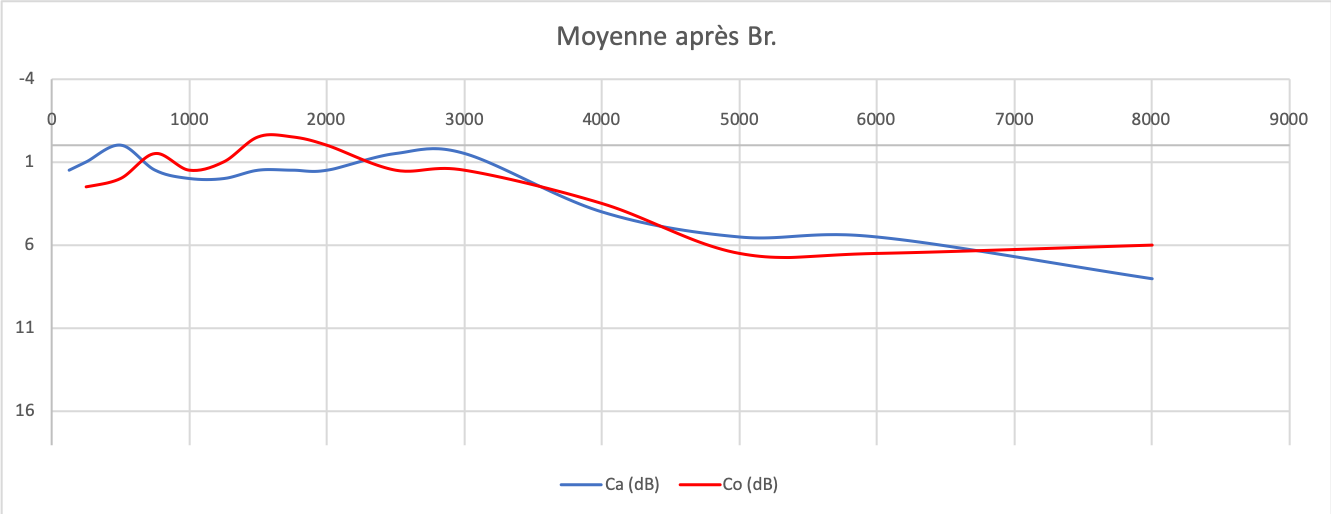
\includegraphics[width=1\linewidth]{images/graphiques/bru_post.png}
\caption[Patient Br. :  2° test]{Second test Br.}

%\label{groupecontroleimage1}
\end{figure}

	\begin{enumerate}
 		\item  c.a.: pas de modification, augmentation des
                  seuils: $-$
 		\item  c.o.: redressement des seuils: $+$
 		\item  croisements: $5/4$ : $+$ : ce qui signifie:  5 croisements lors du 1°test// 4 croisements lors du 2° test= nous avons 1 croisement en moins, donc le résultat est considéré comme positif en fin
                  de séjour.
                \end{enumerate}

                \textbf{ Résultat:  $- $  $+ $   $+ $     :   $+$}
% \clearpage

\paragraph{Patient Sch.:}
\begin{figure}[th]
\centering
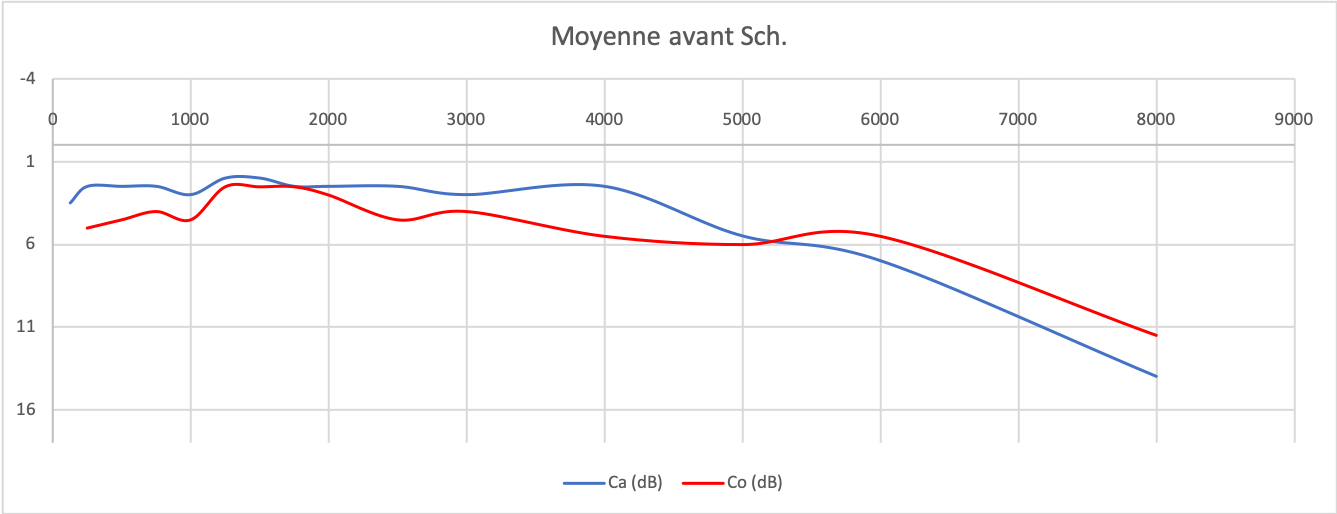
\includegraphics[width=1\linewidth]{images/graphiques/schaff_pre.png}
\caption[Patient Sch. : 1° test]{Premier test Sch.}

%\label{groupecontroleimage1}
\end{figure}


         \begin{figure}[th]
\centering
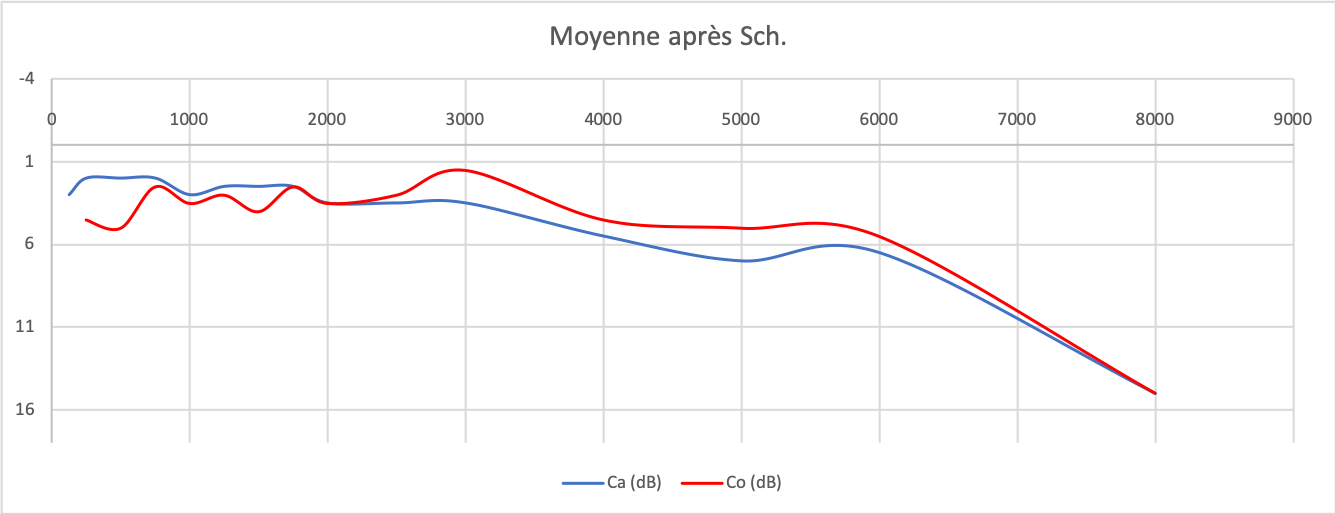
\includegraphics[width=1\linewidth]{images/graphiques/schaff_post.png}
\caption[Patient Sch.: 2° test]{Second test Sch.}

\end{figure}


\begin{enumerate}
	
	\item : c.a.:  modification : +, très légère augmentation puis chute des
	seuils: -
	\item : c.o.: a passé sur c.a. : -, abaissement des seuils:  -
	\item : croisements: 2/1 :     +
\end{enumerate}
\textbf{ Résultat:  $-$    $-$   $+$         :   $-$ }

 \clearpage

\paragraph{ Patient Wal.:}


	\begin{enumerate}

 		\item : c.a.: peu de modification: = ;  seuils: léger redressement: +

 		\item : c.o.:  modification:  + ; reste dominante, tentative de rapprochement de c.a.: +
 		\item : croisements: 1/3 :  -

                \end{enumerate}

                \textbf{ Résultat:  $ + +  -        : +$ }
\begin{figure}[th]
	\centering
	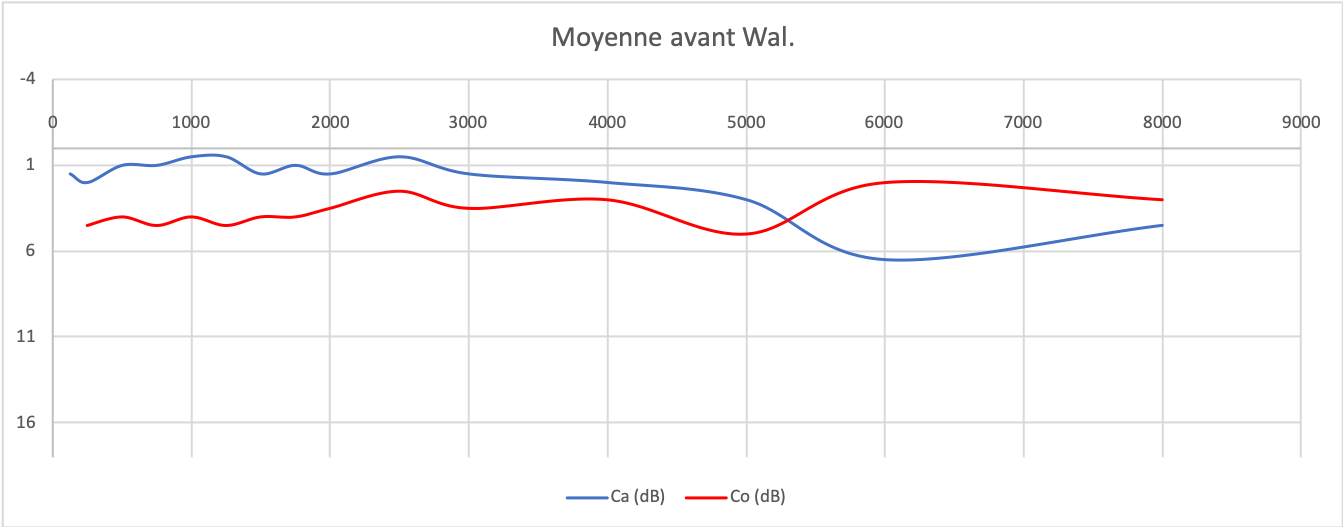
\includegraphics[width=1\linewidth]{images/graphiques/wal_pre.png}
	\caption[Patient Wal. :1° test]{Premier test Wal.}
	
	%\label{groupecontroleimage1}
\end{figure}
               \begin{figure}%[tb]
\centering
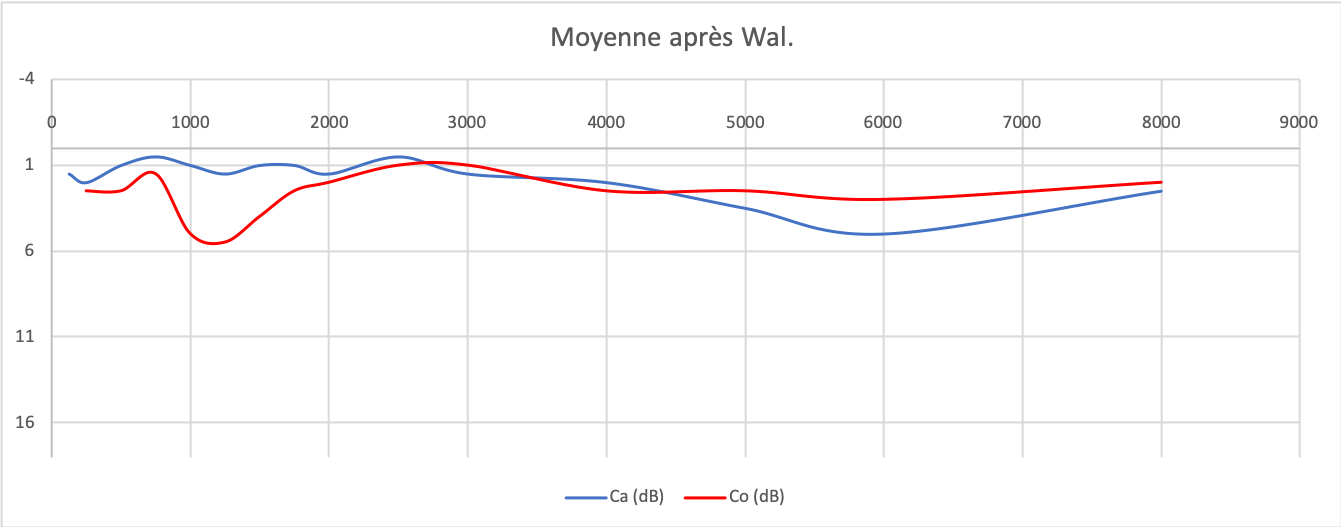
\includegraphics[width=1\linewidth]{images/graphiques/wal_post.png}
\caption[Patient Wal. : 2° test]{Second test Wal.}

\label{groupecontroleimage1}
\end{figure}




\clearpage


\subsection*{Groupe Musicothérapie: observation}
 % \textbf{Groupe de Musicothérapie: }

\paragraph{ Patient Sw.:}



 \begin{figure}[th]
\centering
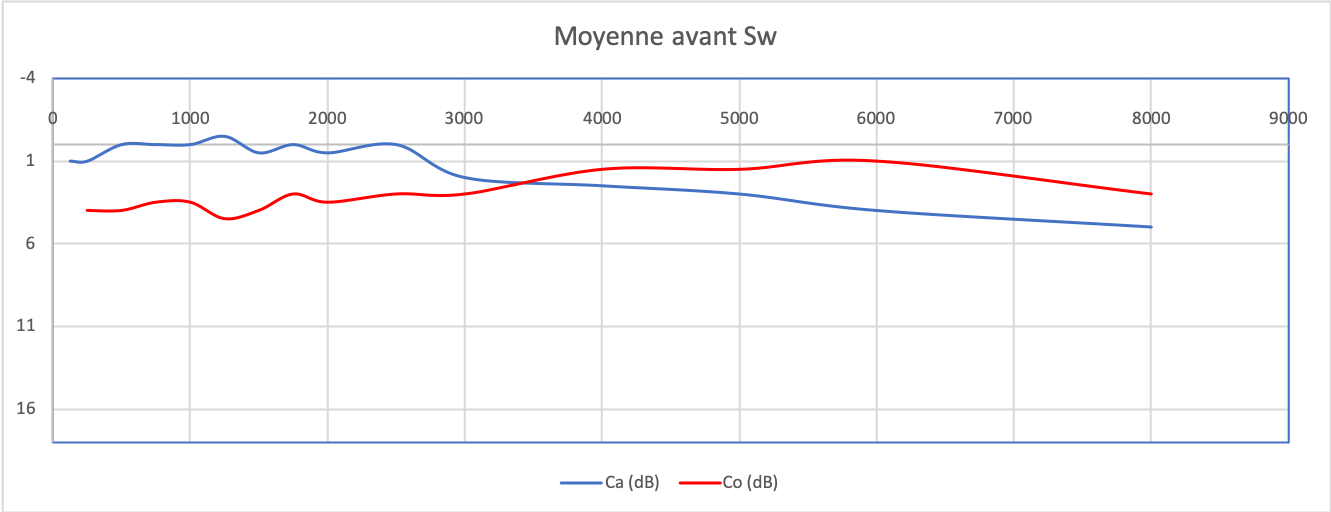
\includegraphics[width=1\linewidth]{images/graphiques/sw_pre.png}
\caption[ \textbf{Groupe Musicothérapie}: Patient Sw. : 1°Test]{Premier test Sw.}

%\label{groupecontroleimage1}
\end{figure}

	\begin{enumerate}

 		\item : c.a.: pas de modification: = %  1,27/1,27

 		\item : c.o.: redressement et rapprochement,
                  relèvement des seuils: -       %  3,07/3,39
 		\item : croisements: 1/3 :  -

                \end{enumerate}

                \textbf{ Résultat:  = +  -        : ``=''}

                \begin{figure}[th]
\centering
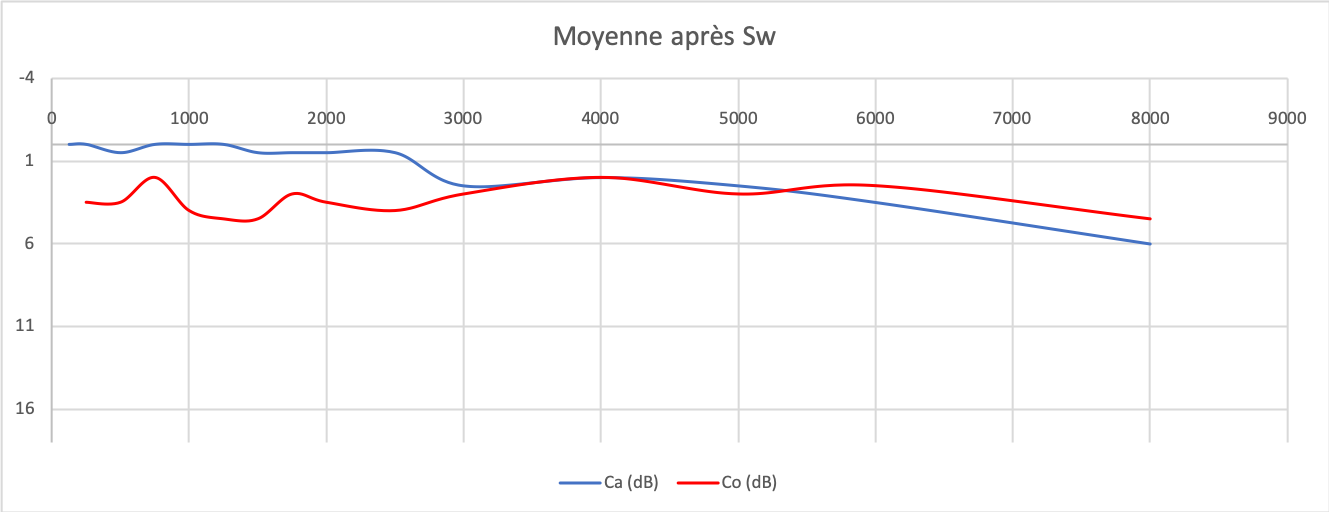
\includegraphics[width=1\linewidth]{images/graphiques/sw_post.png}
\caption[Patient Sw.: 2° test]{Second test Sw.}

%\label{groupecontroleimage1}
\end{figure}


\clearpage

\paragraph{ Patient Cav.: }

(pas de WOQOL fin de séjour)
\begin{figure}%[th]
\centering
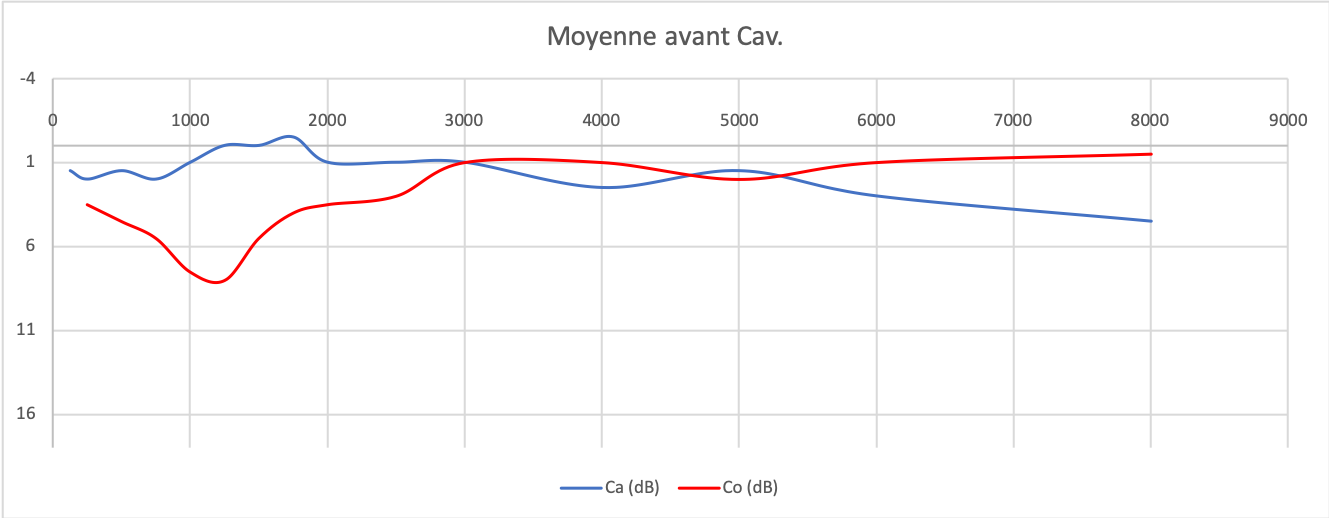
\includegraphics[width=1\linewidth]{images/graphiques/cav_pre.png}
\caption[Patient Cav. : 1° test]{Premier test Cav.}

%\label{groupecontroleimage1}
\end{figure}

	\begin{enumerate}

 		\item : c.a.: redressement: +

 		\item : c.o.: redressement et rapprochement, relèvement des seuils: +
 		\item : croisements: 3/1 :  +

                \end{enumerate}

                \textbf{ Résultat:  + + +       : ``+''}

                \begin{figure}%[th]
\centering
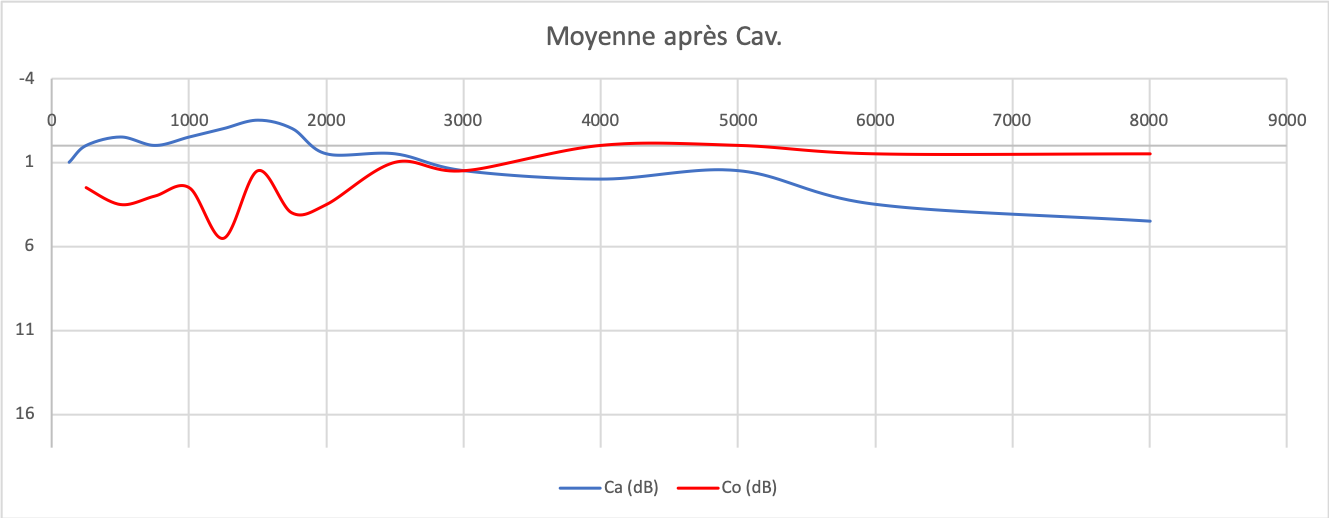
\includegraphics[width=1\linewidth]{images/graphiques/cav_post.png}
\caption[Patient Cav. : 2° test]{Second test Cav.}

%\label{groupecontroleimage1}
                \end{figure}
         \paragraph{ Patient M.:}
	\begin{enumerate}

 		\item : c.a.: redressement: : +   % 6,43/6,03

 		\item : c.o.: redressement et rapprochement,
                  relèvement des seuils:  +     %6,25/5,85:
 		\item : croisements: 3/3 :  =

                \end{enumerate}

                \textbf{ Résultat:  +  +  =     : ``+''}

                \begin{figure}[th]
\centering
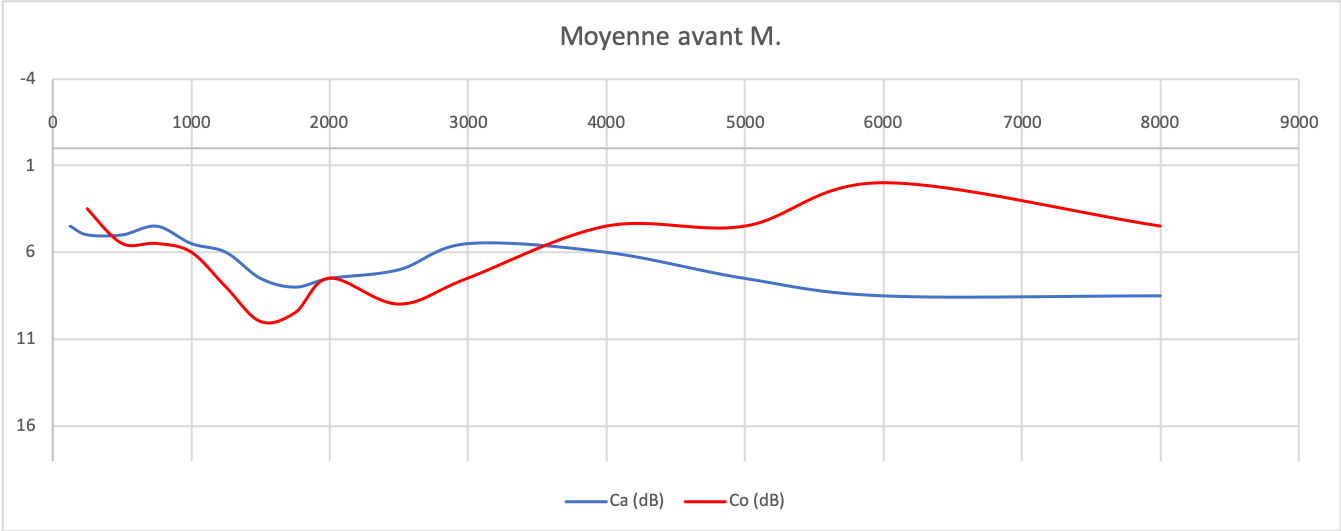
\includegraphics[width=1\linewidth]{images/graphiques/m_pre.png}
\caption[Patient M. : 1° test]{Premier test M.}

%\label{groupecontroleimage1}
\end{figure}


                        \begin{figure}[th]
\centering
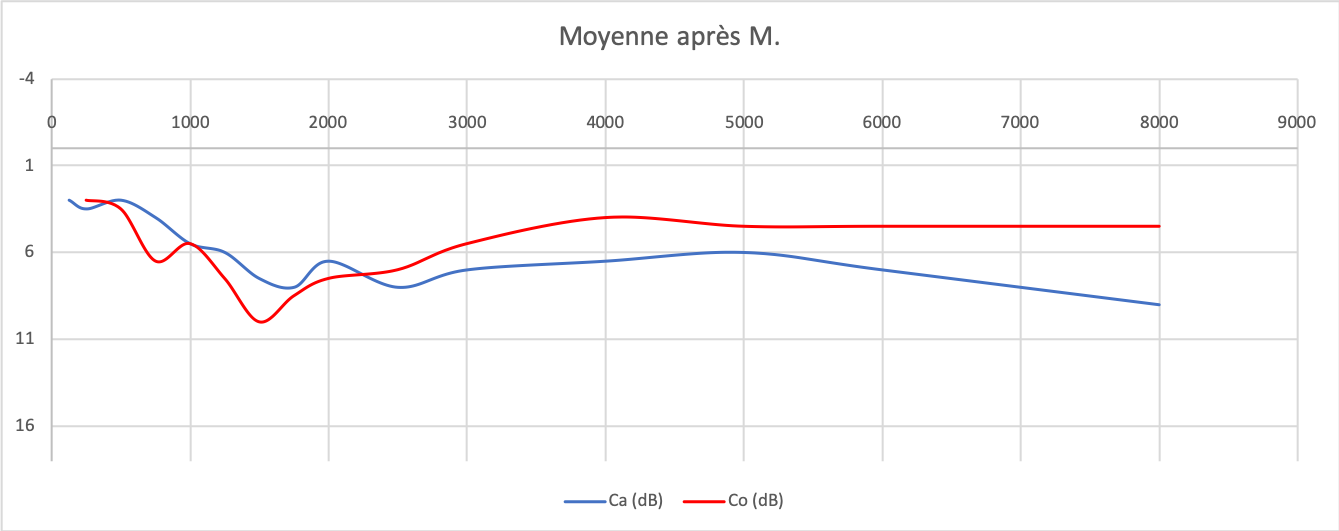
\includegraphics[width=1\linewidth]{images/graphiques/m_post.png}
\caption[Patient M. : 2° test]{Second test M.}

%\label{groupecontroleimage1}
\end{figure}

 

%\section*
\paragraph{Test d'Ecoute: total des résultats du comparatif pré/post-thérapie}
%\textbf{Conclusions générales}:
 : nous nous trouvons
           en présence de deux groupes, un groupe de contrôle et un
           groupe de musicothérapie ayant le même type de
           pathologie -- difficulté de régulation des émotions -- .
Nous constatons, d'une part, que l'écoute est quantifiable.
           D'autre part, il existe bien
          une \textbf{modification de l'écoute pré / post -- traitement}.
Ensuite, il est à observer que
          cette modification est nettement plus marquée
          pour GM, groupe de musicothérapie, qui a un résultat positif.


          \textbf{GM: ``+''}.


Par contre,  pour le groupe de contrôle, GC, le résultat est mitigé, il correspond au signe d'égalité et n'apporte aucune vraie modification.

          \textbf{GC:  ``='' }.


Remarquons que les données quantitatives observables dans
ces graphiques sem\-blent aller dans le
sens de  l'étude faite par le
CNRS  réalisée à partir des seuils auditifs, à savoir
les patients souffrant de troubles post-traumatiques souffrent d'un
\textbf{appauvrissement caractéristique de fréquences} \autocite{affectiveDisorders}.

 
 





















































































%\paragraph{Hypothèse}



%\paragraph{Y-a-t-il une modification de l'écoute du patient après une prise
%en charge en musicothérapie ?}
%Est-ce que le processus d'écoute en musicothérapie améliore la capacité
%d'écoute ? Devient-elle différente après une musicothérapie?

%Est-ce que les test auditifs avant et après la musicothérapie permettent
%de visualiser l'action de la musicothérapie?


%\paragraph{Est-ce que les résultats ($=$ un changement dans l'écoute) d'une prise
%en charge musicothérapeutique peuvent être lisibles et visibles dans
%un test d'écoute?}
%Est-ce possible d'évaluer un travail musicothérapeutique au moyen
%d'un test d'écoute?
%Est-ce que ces résultats sont significatifs?

%\paragraph{Est-ce que l'écoute du patient s'est modifié ? si on a pu observer
%une modification, dans quel sens va -t-elle ?}

%Le contexte:
%est-ce que le contexte est suffisant pour
%ressortir des résultats ?
